% Copyright 2008-2021 by Ning Shang
%
% This is a brief introductory presentation on some mathematics aspects
% of public-key cryptography before and during the first 10 years of the
% 21st century.
%
% This presentation was first given at Professor Bertino's Friday
% ceriasR seminar in 2008, then at an FTO team internal presentation in
% 2009, then was used to fill in a snark hunt schedule in 2011, and then
% was used to fill in a cryptoclub spot.
%
%
%------------------------------------------------------------
% One and only one of the following styles needs to be chosen
%------------------------------------------------------------
%1. Remove comment for projector
\documentclass{beamer}
%
%2. Remove comment for handout
%\documentclass[handout]{beamer}
%
%3. Remove comment for transparency
%\documentclass[trans]{beamer}

%------------------------------------------------------------
\usepackage{amsmath, amsfonts}
\usepackage{beamerthemesplit}
\usepackage{pstricks, pst-plot, pst-tree}
\usepackage{epsfig,graphicx}
\usepackage{algorithm, algorithmic}
% customize algorithm/algorithmic
\renewcommand{\algorithmicrequire}{\textbf{Input:}}
\renewcommand{\algorithmicensure}{\textbf{Output:}}

%\mode<presentation>
%{
%    \usetheme{Warsaw}
%    \usetheme{Pittsburgh}
    \usetheme{Boadilla}
%%    \setbeamercovered{transparent}
     \setbeamercovered{invisible}
%}


% Remove comments for handout
% An alternative way to achieve this is to use the printer options
%\usepackage{pgfpages}
%\pgfpagesuselayout{4 on 1}[letterpaper,border shrink=5mm, landscape]

\title{RSA, ECC, \& Pairing-based Cryptography}
\subtitle{A basic introduction from a math perspective} 

% Insert frame number to footline for Warsaw.
\author
%[Ning Shang\;\hspace{5em} page \insertframenumber]
%[\insertframenumber\;  of\; \inserttotalframenumber \hspace{5em} ]
{ 
Ning Shang 
}

\institute{For filling the void in the cc}

\date{December, 2021}
\begin{document}

\begin{frame}
\titlepage
\end{frame}


%\begin{frame}{Outline}
%\tableofcontents[pausesections]
%\end{frame}

%-- Section: Cryptography overview --
\section{Overview of Cryptography}
%--Page: Overview of crypto --
\begin{frame}{}
\begin{figure}[htbp]
\centering
  
\includegraphics[width=\textwidth]{img/chap1-overview-crypto.pdf}
\end{figure}
\end{frame}

%-- Page: overview of cryptography --
\begin{frame}{Cryptography: Overview}
    \begin{block}{What is cryptography?}
    \emph{Study of mathematics techniques related to aspects of information
security, e.g., how to hide information, data integrity, identification and
authentication.}
    \end{block}
\end{frame}

\begin{frame}{Cryptography: Overview (cont'd)}
\begin{figure}[htbp]
\centering
  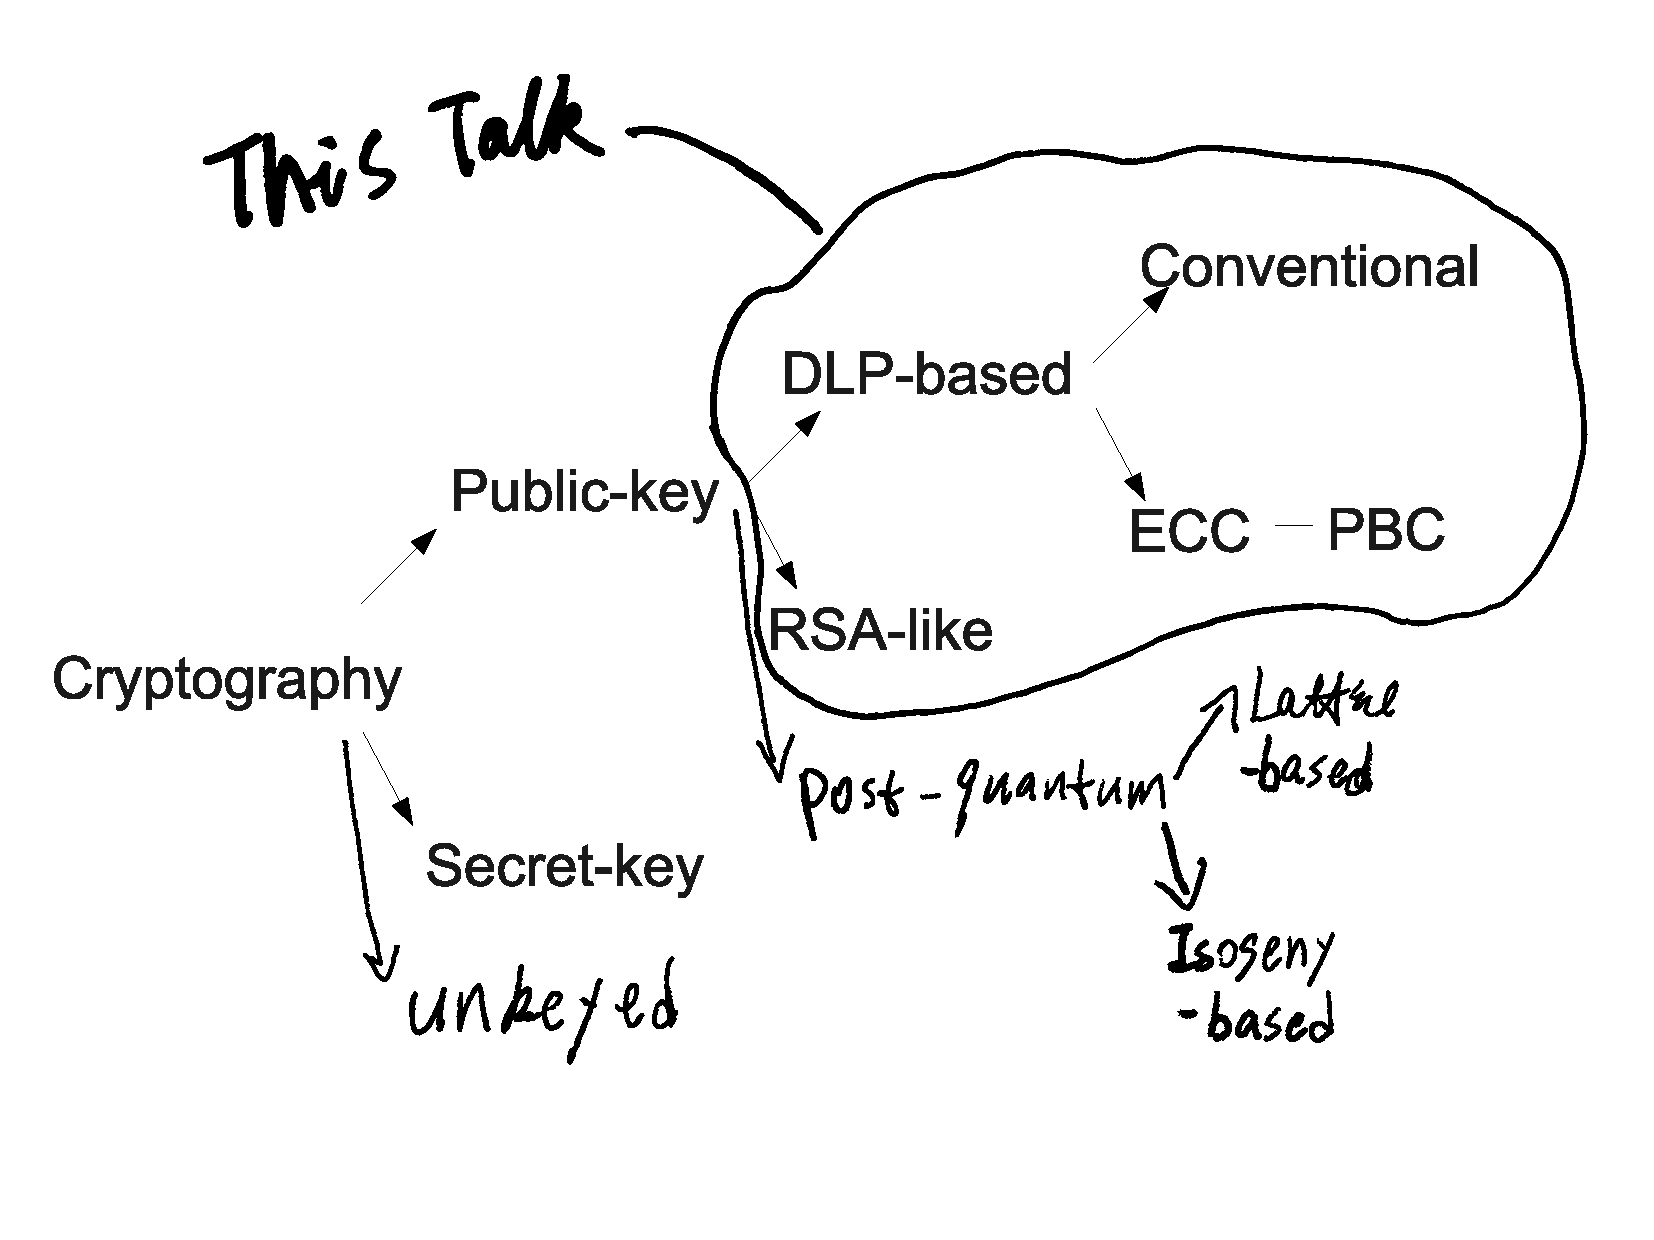
\includegraphics[width=0.9\textwidth]{img/cryptotree.pdf}
  \caption{A tree view of cryptography}
  \label{fig:cryptotree}
\end{figure}

\end{frame}

%-- Section: RSA --
\section{Rivest-Shamir-Adleman (RSA)}
%-- Page: RSA --
\begin{frame}{}
\begin{figure}[htbp]
\centering
  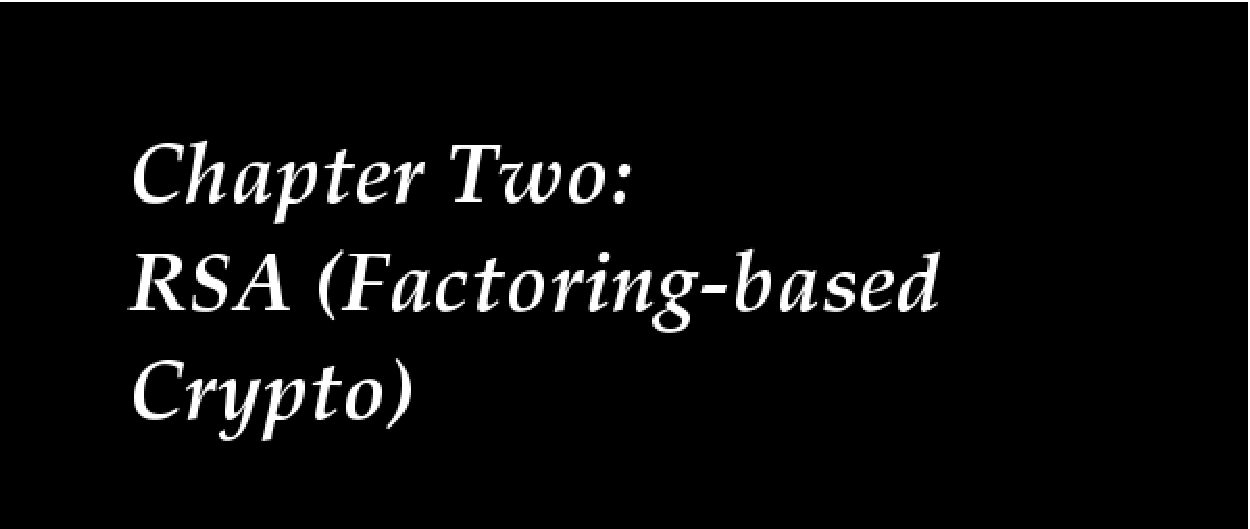
\includegraphics[width=\textwidth]{img/chap2-rsa.pdf}
\end{figure}
\end{frame}

%-- Page: Intractability of factorization --
\begin{frame}{Rivest-Shamir-Adleman}
Setup/KeyGen:
\begin{itemize}
\item[-] Choose two large primes $p$ and $q$.
\item[-] Let $n = p \cdot q$.
\item[-] Randomly choose $e$ such that $1< e < n-1$ and $\gcd(e, \phi(n)) = 1$. 
Here $\phi(n) = (p-1)(q-1)$ is the Euler's totient function.
\item[-] Compute $d$ such that $e\cdot d \equiv 1 \pmod{\phi(n)}$.
\item[-] The values $p$ and $q$ are never revealed.
\end{itemize}

\begin{block}{}
RSA public key: $(n, e)$.

RSA private key: $d$.
\end{block}

\vskip 10pt

Remark: for RSA to work, factorization of the modulus $n$ should be hard.
\end{frame}

%-- Page: RSA encryption --
\begin{frame}{RSA Encryption (Basic Scheme)}
\begin{block}{}
Plaintext message: $M\in\left\{1, 2, \ldots, n-1\right\}$.

Encryption: $C := E(M) = M^e \pmod{n}$.

Decryption: $M := D(C) = C^d \pmod{n}$.
\end{block}
\end{frame}

%-- Page: RSA signature --
\begin{frame}{RSA Signatures (Basic Scheme)}

\begin{block}{}
Message to sign: $M \in\left\{1, 2, \ldots, n-1\right\}$.

Sign: signature $\sigma = D(M) = M^d \pmod{n}$.

Verify: check $M = E(\sigma) = \sigma^e \pmod{n}$.
\end{block}

Remark: The scheme shown above is not secure.  In practice, one should
sign the hash of the message instead of the message itself.

\end{frame}

%-- Section: ECC --
\section{Elliptic Curve Cryptography (ECC)}
%-- Page: ECC --
\begin{frame}{}
\begin{figure}[htbp]
\centering
  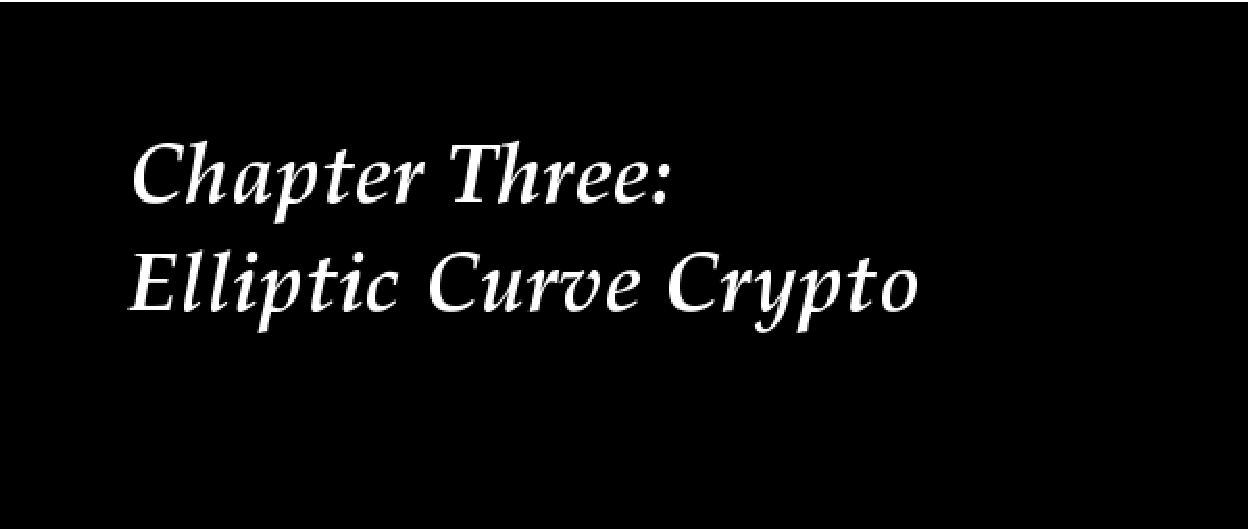
\includegraphics[width=\textwidth]{img/chap3-ecc.pdf}
\end{figure}
\end{frame}

\begin{frame}{Elliptic Curves in Cryptography}
Application of elliptic curves in cryptography
\begin{itemize}
\item<1-> Public-key encryption and signature algorithms (ECC)
\item<2-> Integer factorization method (ECM)\quad~\cite{Lenstra1987}
\item<3-> Primality test (ECPP)\quad~\cite{AdHu1987}
%\item<4-> Identity-based encryption (IBE)\quad~\cite{BoFr2003}
\item<4-> Key management schemes\quad~\cite{BeShWa2008}
\item<5-> Hash function construction\quad~\cite{ChGoLa2007}
\item<6-> Zero-knowledge proofs
\item<7-> And so on
\end{itemize}
\end{frame}

%-- Page: Lang's quote --
\begin{frame}{A Mathematician Quote}
\begin{center}
 {\Large ``It is possible to write endlessly on elliptic curves. (This is not 
a threat.)''
\hfill --- Serge Lang}
\end{center}
\end{frame}

%-- Page: focus on ECC
\begin{frame}{We Follow The Wise}
We are not going to talk about everything ...

\begin{block}{Focus of this talk: ECC}
Elliptic curve cryptography: use elliptic curves as an approach to public-key 
cryptography
\end{block}
\end{frame}

%-- Subsection: applications of elliptic curves in cryptography --
\subsection{Ellipituc Curves in Cryptography}

%-- Page: EC definition, illustration
\begin{frame}{Elliptic Curve}
\begin{center}
{\Large 
$E: y^2 = x^3 + a x + b, \quad a, b\in \mathbb{F}_q$, $q$ odd $3 \nmid q$
}
\end{center}
\begin{figure}[htbp]
\centering
  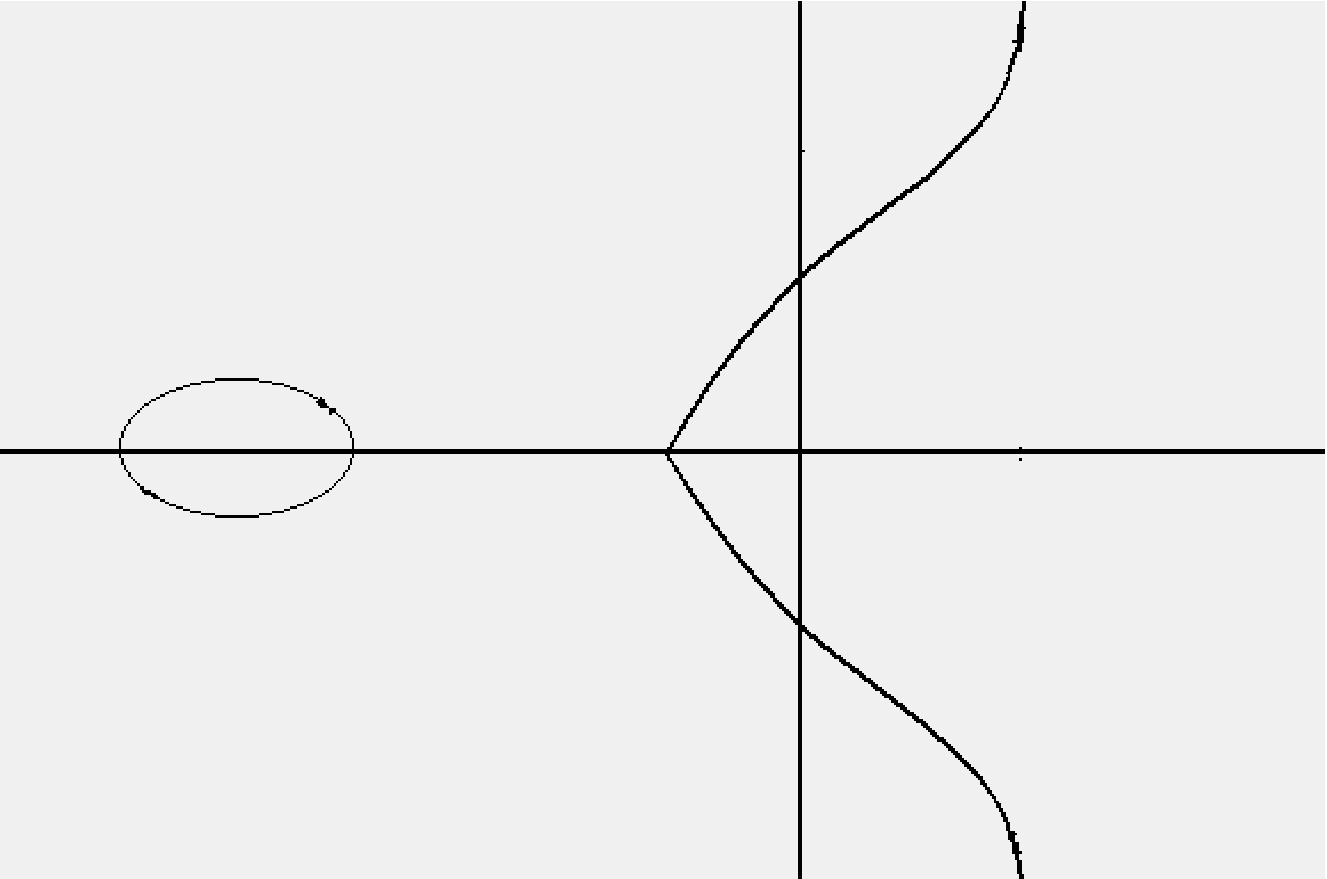
\includegraphics[width=0.6\textwidth]{img/ecurve.pdf}
  \caption{An example of elliptic curve over $\mathbb{R}$}
  \label{fig:ecurve}
\end{figure}

\end{frame}


\subsection{ECC}
%-- Page: review group --
\begin{frame}{Review: Group}
A group is a set $G$ together with a binary operation $\circ$ that satisfies
\begin{enumerate}
\item closure: $a, b\in G \Rightarrow a\circ b \in G$
\item associativity: for any $a, b, c\in G$, have $(a\circ b)\circ c 
= a\circ (b\circ c)$
\item identity: there exists an identity element $i$ such that 
$a\circ i = i\circ a = a$, for any $a\in G$
\item inverse: for any element $a\in G$, there is an element $b\in G$ such
that $a\circ b = b\circ a = i$. 
\end{enumerate}
\end{frame}

\begin{frame}{Review: Group (cont'd)}
\begin{block}{Abelian Group}
A group $G$ is called {\bf abelian} if $a\circ b = b\circ a$, for any 
$a, b\in G$.
\end{block}

\begin{block}{Examples of abelian groups}
- ($\mathbb{Z}, +)$\\
- ($\mathbb{F}_p^{\times}, \cdot$)\\
- ($E(\mathbb{F}_q), +)$: elliptic curve over finite field
\end{block}

Finite abelian groups are convenient for cryptography, because the group law
behaves well!  

\alert{No need to worry about things like $a + b \ne b + a$}

\end{frame}

%-- Page: DLP based crypto --
\begin{frame}{Discrete Logarithm Problem} 
\begin{block}{Discrete logarithm problem (DLP)}
    $G = \langle\alpha\rangle$: finite cyclic group of order N with generator
$\alpha$; written multiplicatively. $\beta = \alpha^n$ for some $n \in \{0, 1,
2, \ldots, N - 1\}$.\\
    DLP: given $\alpha, \beta$, find $n$.
\end{block}

\end{frame}

\begin{frame}{Discrete Logarithm Problem (cont'd)}
\begin{block}{Example}
$G = \left(\mathbb{Z}/(1152921504606847363)\right)^{\times} =
\langle\alpha\rangle, \alpha = \overline{12345678}$. \\
Given $n = 64051194700380044$, it is easy to compute 
$\beta = \alpha^n =
\overline{24306907499566794}$: \quad $O(\log N)$. \\
If only $\alpha = \overline{12345678}$ and $\beta =
\overline{24306907499566794}$ are given, how to recover $n$?
\end{block}
\end{frame}

\begin{frame}{Discrete Logarithm Problem (cont'd)}
\setbeamercovered{invisible}
\onslide<1>{\Large
\alert{Bad news: this is in general a hard problem.}\\
Best generic methods take time $O(\sqrt{N})$ -- Shank's BSGS, Pollard's 
$\rho$ and $\lambda$ methods.
}

\pause
\vskip .5in

\alert{\Large Good news: we can use it to do cryptography!}
\end{frame}

\begin{frame}{Discrete Logarithm Based Cryptography}

\begin{block}{Example: Diffie-Hellman(-Merkle) key exchange protocol}
    Enables two parties to share a common secret (e.g. an symmetric encryption
key) over an insecure communications channel.

    How it works:
\begin{enumerate}
    \item Alice and Bob agree on a finite cyclic group $G$ and a generator
$\alpha$. 
    \item Alice chooses a secret integer $m$, computes $\beta = \alpha^m$, and
sends $\beta$ to Bob.
    \item Bob chooses a secret integer $n$, computes $\gamma = \alpha^n$, and
sends $\gamma$ to Alice.
    \item Alice computes $\gamma^m = \alpha^{nm}$; Bob computes $\beta^n =
\alpha^{mn}$; this information is used as their shared secret.
\end{enumerate}
\end{block}
\end{frame}

%-- Page: choice of finite group for DLP --
\begin{frame}{Groups Suitable for DLP Based Cryptography}
\begin{block}{Requirements}
\begin{itemize}
\item Intractability of DLP: \\
    - group order is desired to be ``almost prime'': to resist the
Pohlig-Hellman attack. \\
    - No ``easy'' transformation into another group where DLP can be solvable
in less time: to resist attacks like MOV, GHS, ...
\item Compact representation of group elements.
\item Efficient group operations.
\end{itemize}
\end{block}
\end{frame}

\begin{frame}{Group Suitable for DLP Based Cryptography (cont'd)}
    Candidates:
\begin{itemize}
\item Multiplicative groups of finite fields $\mathbb{F}_q^{\times}$.
\item Class groups of orders in number fields.
\item Abelian varieties over finite fields, e.g., Jacobians of algebraic
curves, {\bf ELLIPTIC CURVES}.
\item Others.
\end{itemize}
\end{frame}

%-- Page: use elliptic curve for DLP based cryptography --
\begin{frame}{Elliptic Curve Group}
\begin{center}
Elliptic curve
{\Large 
$E: y^2 = x^3 + a x + b, \quad a, b\in \mathbb{F}_q$, $q$ odd, $3\nmid q$
}
\end{center}

$\mathbb{F}_q$-rational points of $E$, 
$$E(\mathbb{F}_q) := \{(x, y)\in (\mathbb{F}_q)^2: y^2 = x^3 + a x + b\}\cup 
\{\infty\}$$

\pause
\begin{block}{Important fact about $E(\mathbb{F}_q)$}
$E(\mathbb{F}_q)$ is a finite abelian group

\alert{NON-TRIVIAL! Do Not Try This at Home!}
\end{block}

Group operation in $E(\mathbb{F}_q)$ is often written as addition (+)\\
Scalar multiplication: 
$[m]P :=\underbrace{P + P + \ldots + P}_{m\textrm{ times}}$

\end{frame}

% ECDH
\begin{frame}{Elliptic Curve Diffie-Hellman(-Merkle) key exchange}
Rewrite Diffie-Hellman key exchange in language of elliptic curves.

\begin{enumerate}
    \item Alice and Bob agree on an elliptic curve $E(\mathbb{F}_q)$ and 
a point $P\in E(\mathbb{E}_q)$ as base point. 
    \item Alice chooses a secret integer $m$, computes $Q = [m]P$, and
sends $Q$ to Bob.
    \item Bob chooses a secret integer $n$, computes $R = [n] P$, and
sends $R$ to Alice.
    \item Alice computes $[m]R = [nm]P$; Bob computes $[n]Q =
[mn]P$; this information is used as their shared secret.
\end{enumerate}

\end{frame}

 % Page: group law illus
\begin{frame}{Group Operation in $E(\mathbb{F}_q)$}


\begin{center}
{\Large 
$E: y^2 = x^3 + a x + b, \quad a, b\in \mathbb{F}_q$, $q$ odd, $3\nmid q$
}
\end{center}
\begin{figure}[htbp]
\centering
  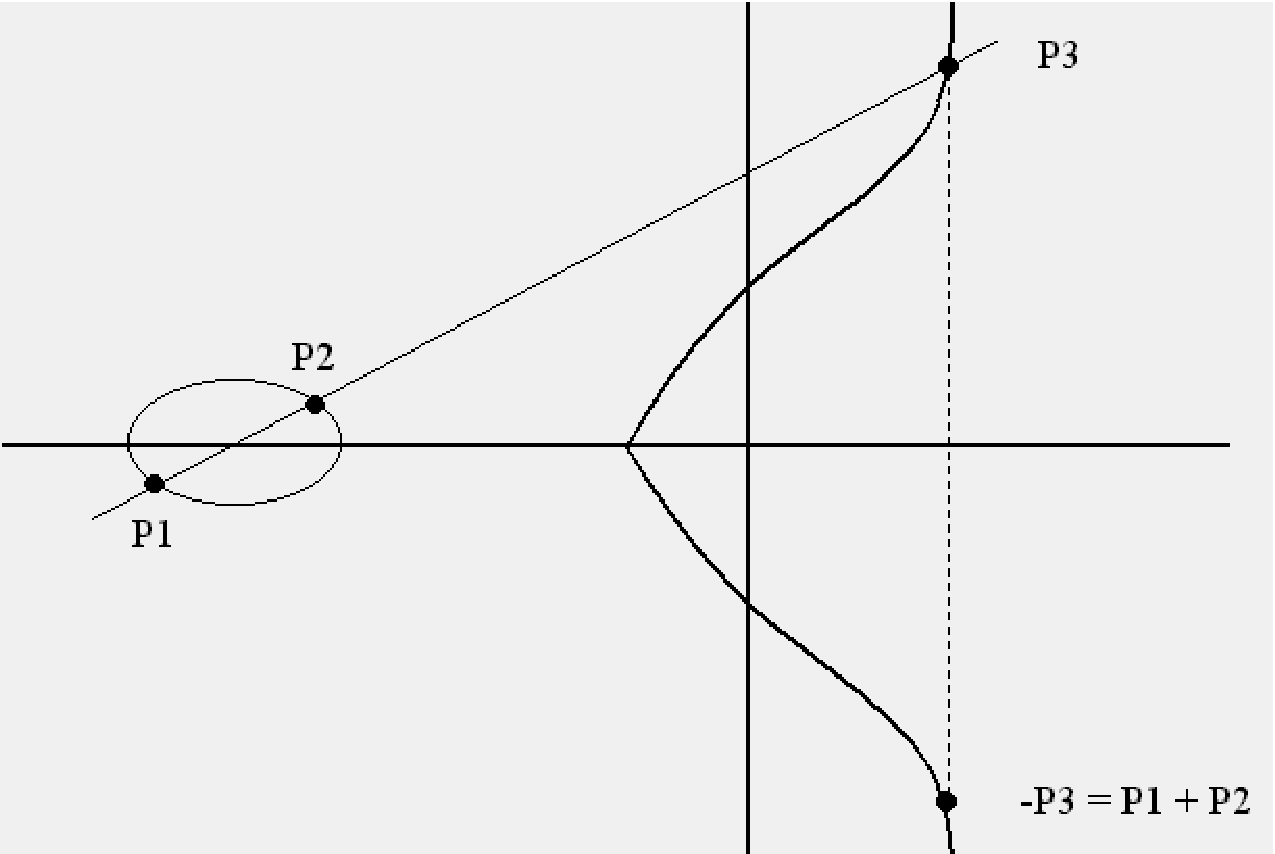
\includegraphics[width=0.6\textwidth]{img/ecurve_arith.pdf}
  \caption{Illustration of points addition (courtesy of \sf{garykessler.net})}
  \label{fig:ecurve_arith}
\end{figure}

\end{frame}

\begin{frame}{Group Law for $E(\mathbb{F}_q)$}
Input: $P_1(x_1, y_1), \quad P_2(x_2, y_2)$\\
Output $Q(x, y) = P_1 + P_2$

\begin{block}{Case $P_1 \ne P_2$: I, 3M/S}
\begin{align*}
\lambda & = (y_2 - y_1)/(x_2 - x_1) \\
x & = \lambda^2 - x_1 - x_2 \\
y & = (x_1 - x)\lambda - x - y_1
\end{align*}
\end{block}

\begin{block}{Case $P_1 = P_2$: I, 4M/S}
\begin{align*}
\lambda & = (3x_1^2 + a)/(2y_1) \\
x & = \lambda^2 - 2 x_1 \\
y & = (x_1 - x)\lambda - x - y_1
\end{align*}
\end{block}
\end{frame}

%-- Advantage of EC
\begin{frame}{Elliptic curve $E(\mathbb{F}_q)$ vs. $\mathbb{F}_p^{\times}$}
\large Reason to replace ``conventional'' choice of the multiplicative group 
$\mathbb{F}_p^{\times}$?
~\\[.5in]
\pause
\begin{center}
\textcolor{blue}{\bf\Huge EFFICIENCY}
\end{center}

At same level of security, crypto schemes implemented with elliptic
curves run faster than their $\mathbb{F}_q^{\times}$ counterparts, with
much shorter key lengths.
\end{frame}

\begin{frame}{Elliptic curve $E(\mathbb{F}_q)$ vs. $\mathbb{F}_p^{\times}$ 
(cont'd)}
 $n$: bit length of $q$

 $N$: bit length of $p$

\begin{block}{Complexity of best known attacks to DLP}
- Elliptic curve $E(\mathbb{F}_q)$: 
$$C_{\mathrm{ec}} = 2^{n/2}$$

- Multiplicative group $\mathbb{F}_q^{\times}$: 
$$C_{\mathrm{conv}} = \exp(1.92 N^{1/3} (\log(N \log 2))^{2/3})$$

\end{block}
\end{frame}

\begin{frame}{Elliptic curve $E(\mathbb{F}_q)$ vs. $\mathbb{F}_p^{\times}$ 
(cont'd)}
\begin{block}{Crude Estimate}
$C_{\mathrm{ec}} = C_{\mathrm{conv}} \Longrightarrow 
n = 4.91 N^{1/3} (\log(N \log 2))^{2/3}$
\end{block}

\begin{figure}[htbp]
\centering
  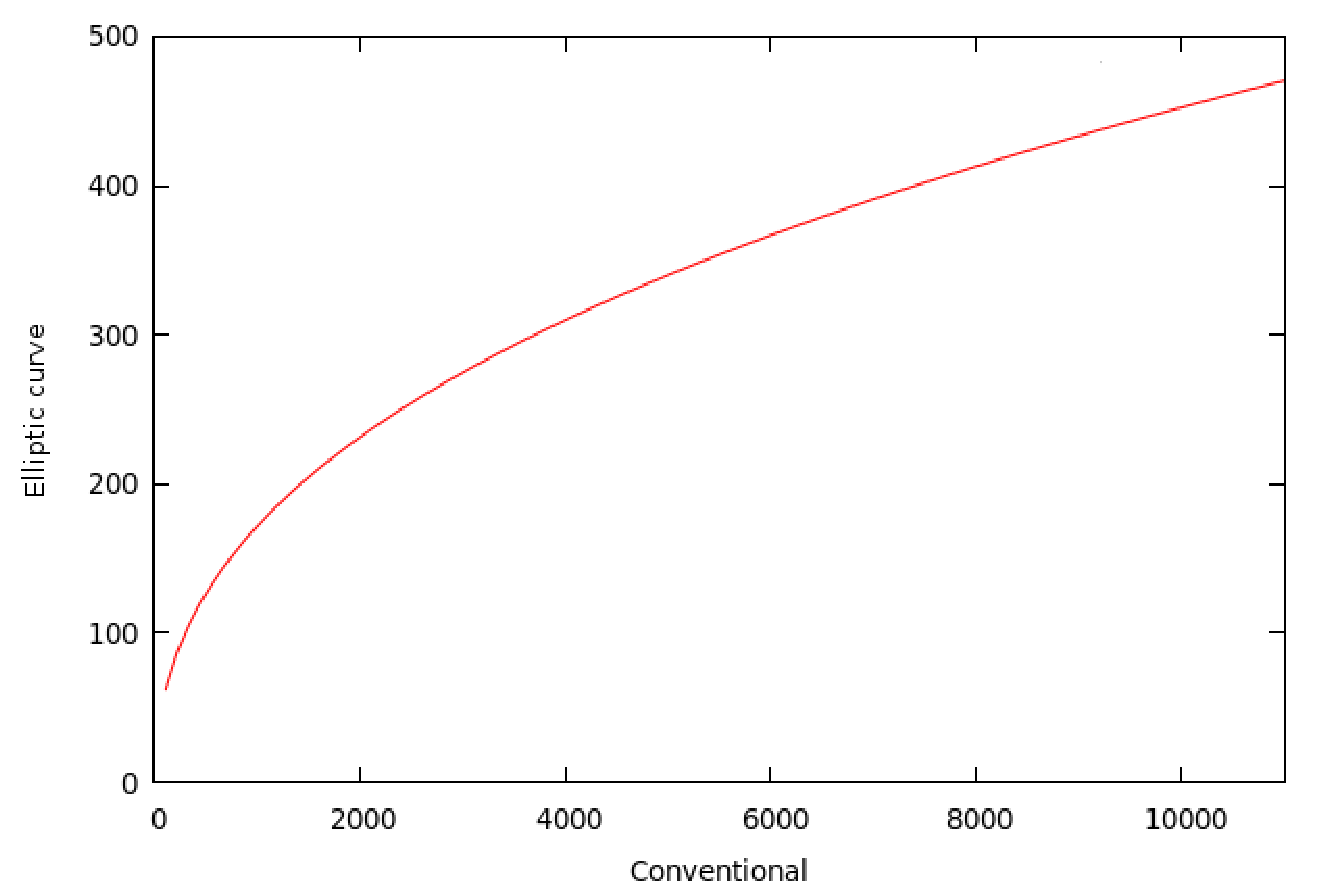
\includegraphics[width=0.6\textwidth]{img/ec_Fp_cmp.pdf}
  \caption{Elliptic curve vs. $\mathbb{F}_p^{\times}$ key sizes (in bits)
for similar security level}
  \label{fig:ec_Fp_cmp}
\end{figure}

\end{frame}

\begin{frame}{Elliptic Curve $E(\mathbb{F}_q)$ vs. $\mathbb{F}_p^{\times}$ (cont'd)}
Estimate above tells us
~\\[.3in]
\begin{tabular}{|p{1in}|p{1in}|p{1in}|}
\hline
bit-strength & size $q$ (bits) & size $p$ (bits) \\\hline
87  & 173 & 1024\\\hline
117 & 233 & 2048 \\\hline
157 & 313 & 4096 \\\hline
209 & 417 & 8192 \\\hline
\end{tabular}
~\\[.3in]

The estimate is at best crude, but it at least gives us some ideas about the
low-costness of ECC over conventional public-key cryptosystems.

\end{frame}

\begin{frame}{Elliptic Curve vs. RSA}
\begin{block}{}
Similar arguments apply to cryptosystems based on RSA.
\end{block}
~\\[.3in]

\pause

In practice, the performance comparison relies on implementation.

\begin{block}{Commercial Time}
In the commercial cryptographic literature, \\
1024-bit RSA $\approx$ 160-bit ECC~\cite{LeVe2001}.
\end{block}

\end{frame}


%-- Page: compare DSA with ECDSA, case study
\begin{frame}{DSA vs. ECDSA}
$q$: order of prime field $\mathbb{F}_q$\\
$r$: order of subgroup of $\mathbb{F}_r^{\times}$\\
$n$: order of subgroup of $E(\mathbb{F}_p)$\\
$h$: cofactor such that $|E(\mathbb{F}_p)| = n\cdot h$\\

~\\[.2in]

The Digital Signature Standard (FIPS PUB 186-3) recommends\\
{\bf DSA}\\
\begin{tabular}{|p{.7in}|p{.7in}|p{.7in}|p{.7in}|p{.7in}|}
\hline
size $q$ & 1024 & 2048 & 2048 & 3072 \\\hline
size $r$ & 160 & 224 & 256 & 256\\
\hline
\end{tabular}
~\\[.1in]

{\bf ECDSA}\\
\begin{tabular}{|p{.4in}|p{.6in}|p{.6in}|p{.6in}|p{.6in}|p{.6in}|}
\hline
size $n$ & 161-223 & 224-255 & 256-383 & 384-511 & $\ge 512$\\\hline
max $h$ & $2^{10}$ & $2^{14}$ & $2^{16}$ & $2^{24}$ & $2^{32}$\\
\hline
\end{tabular}
\end{frame}

%-- Page: real world --
\begin{frame}{In Real World}
Elliptic curve cryptography
\begin{itemize}
\item Elliptic curve based public-key cryptography is part of NSA Suite B.
\item ECC has been written into various industrial standards
eg. Digital Signature Standard (FIPS PUB 186-3).
\item ECC has been integrated in many software and hardware (eg. latest version
of OpenSSL, NSS v3.8, Firefox).
\item A number of companies dedicated to ECC (eg. Certicom)
\item Numerous white papers, presentations and publications (of course)
\end{itemize}
\end{frame}

%-- Section: PBC --
\section{Pairing-Based Cryptography (PBC)}
%-- Page: PBC --
\begin{frame}{}
\begin{figure}[htbp]
\centering
  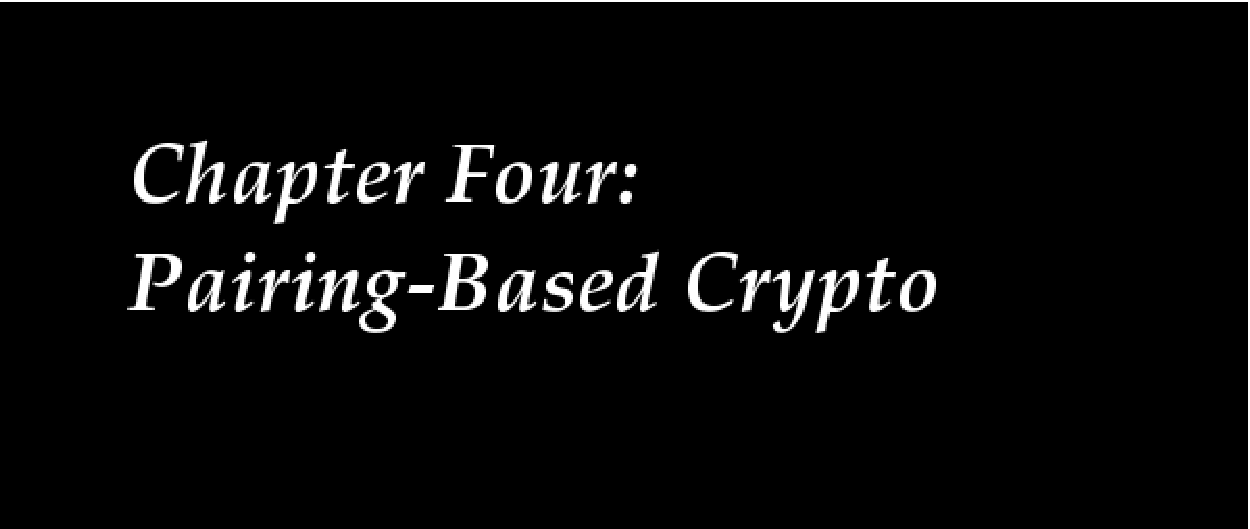
\includegraphics[width=\textwidth]{img/chap4-pbc.pdf}
\end{figure}
\end{frame}

%-- Page: pairings
\begin{frame}{Beyond Efficiency: Bilinear Maps}
Many useful cryptographic protocols and applications, eg. IBE, short 
signatures, aggregate signatures, require use of a bilinear map
$$e: G_1 \times G_2 \rightarrow G_T$$

\begin{block}{Bilineality}
For all $P_1\in G_1$, $P_2 \in G_2$, $m, n\in \mathbb{Z}$, 
$e([m]P_1,[n]P_2) = e(P_1, P_2)^{mn}$
\end{block}

\begin{block}{Non-degeneracy}
For $\mathcal{O}\ne P_1\in G_1$, there exists $P_2\in G_2$ such that
$e(P_1, P_2) \ne 1$
\end{block}
\end{frame}

%\begin{frame}{Beyond Efficiency: Bilinear Maps (cont'd)}
%With efficient implementation of bilinear maps, we have groups in which the 
%Decision Diffie-Hellman problem (DDH) is easy, and the Computational 
%Diffie-Hellman problem (CDH) remains hard.
%
%\begin{block}{Decision Diffie-Hellman (DDH)}
%Given $P, [m]P,[n]P, Q \in G$, decide whether $Q = [m + n] P$
%\end{block}

%With $e: G_1 \times G_2 \rightarrow G_T$, have
%$Q = [m + n] Q \Leftrightarrow e(Q, P) = e([m]P, P) e([n]P, P)$.

%\begin{block}{Computational Diffie-Hellman (CDH)}
%Given $P, [m]P, [n]P\in G$, compute $[m + n] P$
%\end{block}
%
%
%Similarly, we have Decision co-Diffie-Hellman and Computational 
%co-Diffie-Hellman (useful for aggregate signatures).
%\end{frame}


\begin{frame}{Beyond Efficiency: Bilinear Maps (cont'd)}
For certain kinds of elliptic curves, there exist efficient implementation
of bilinear maps -- the elliptic curve pairings (eg. Weil pairings, 
Tate pairings, Ate pairings, $\ldots$)
$$e: G_1 \times G_2 \rightarrow G_T$$

$G_1$ and $G_2$ are subgroups of $E(\mathbb{F}_q)$, $G_T$ is a subgroup of 
$\mathbb{F}_{q^k}^{\times}$ for some small integer $k$. 
$|G_1| = |G_2| = |G_T| = r$.

\begin{block}{}
Elliptic curve pairings are so far the only known efficient implementation
of bilinear maps suitable for cryptography.
\end{block}
\end{frame}

\begin{frame}{Miller's algorithm for Tate pairings}

{\footnotesize
\begin{algorithm}[H]
\caption{Basic Miller's algorithm}
\begin{algorithmic}[1] % to number every line
\REQUIRE $P\in G_1 \subseteq E(\mathbb{F}_{q^k}), Q\in G_2 \subseteq 
E(\mathbb{F}_{q^k})$, where $r$ is the order of $P$
\ENSURE $e(P, Q)$

\STATE $T\leftarrow P, f\leftarrow 1$
\FOR {$i=\lfloor \lg(r) \rfloor - 1$ to $0$}
\STATE $f = f^2\cdot l_{T, T}(Q)/v_{2T}(Q)$
\STATE $T = 2T$
\IF {the $i$-th bit (from right) of $r$ is $1$}
 \STATE $f = f\cdot l_{T, P}(Q)/v_{T+P}(Q)$
 \STATE $T = T + P$
\ENDIF
\ENDFOR
% final exponentiation
\STATE $f\leftarrow f^{(p^k - 1)/r}$
%
\RETURN $f$
\end{algorithmic}
\end{algorithm}
Here $l_{A, B}(Q)$ and $v_{A+B}(Q)$ are the ``line'' and ``vertical'' functions,
resp.
}
\end{frame}

\begin{frame}{Elliptic Curves Suitable for PBC}
``Pairing-friendly curves''
\begin{itemize}
\item[-] Present additional mathematical structures.
\item[-] Provide additional crypto hardness assumptions.
\item[-] Must satisfy all requirements for (regular) ECC.
\item[-] Have low density in all elliptic curves suitable for ECC
\end{itemize}
\end{frame}

\begin{frame}{Applications of PBC}

You cannot do (or do better) the following things without PBC.

\begin{itemize}
\item[-] Tripartite key exchange~\cite{Joux2000} 
% Intractability assumption: decision bilinear Diffie-Hellman problem (DBDHP)
\item[-] Identity-based encryption (IBE)~\cite{BoFr2003}, 
attributed-based encryption (ABE)
% Intractability assumptions: DBDHP/computational bilinear Diffie-Hellman 
% problem (CBDHP)
\item[-] Short signature scheme~\cite{BLS2001} 
% Intractability assumption: Gap-DH
\item[-] Aggregate signature scheme with different signing keys~\cite{BGLS2003}
% Intractability assumption: Co-Gap-DH (case G1 <> G2)
\item[-] Efficient non-interactive zero-knowledge proofs \cite{GrSa2008}
% Intractability assumptions: subgroup decision assumption (SD)/symmetric 
% external Diffie-Hellman (SXDH)/decisional linear assumption (DLIN)
\item[-] Broadcast encryption scheme \cite{BoWa2006}

\end{itemize}
\end{frame}



%-- Page: end
\begin{frame}{}
\begin{figure}[htbp]
\centering
  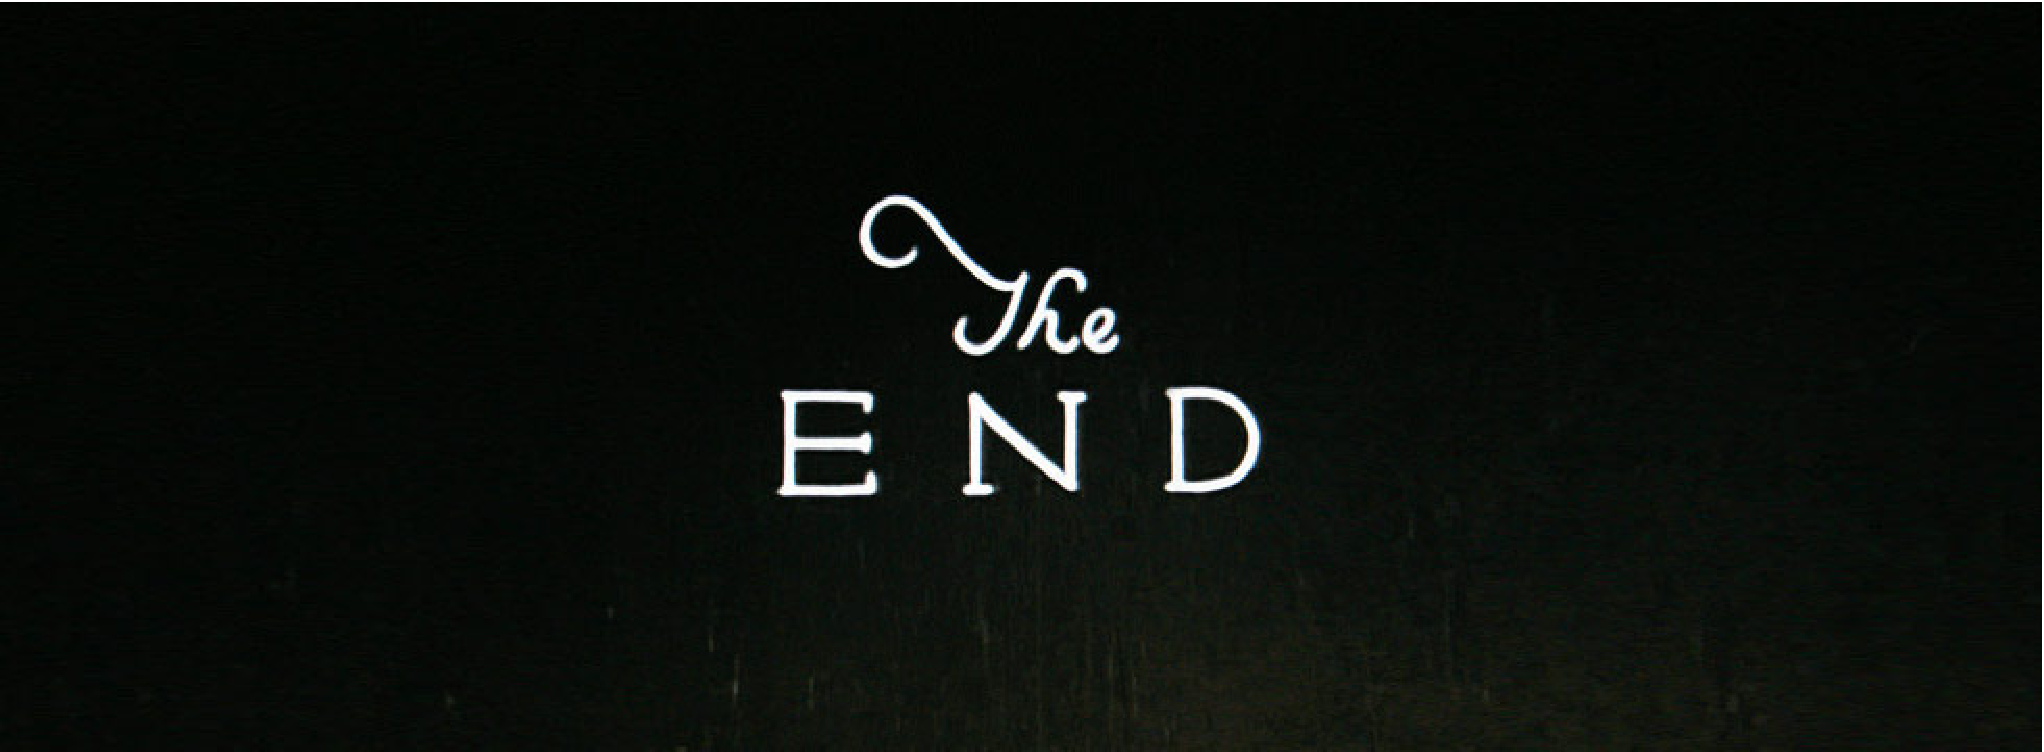
\includegraphics[width=\textwidth]{img/TheEnd.pdf}
\end{figure}
\end{frame}

%-- References --
\begin{frame}[allowframebreaks]{References}
\tiny
\bibliographystyle{apalike}
\bibliography{bibecc}
\end{frame}
\end{document}
